\documentclass{standalone}
\usepackage{pgf, tikz}
\usetikzlibrary{arrows, automata}
\begin{document}
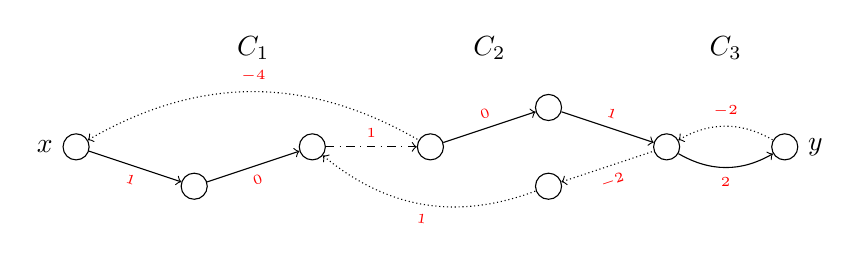
\begin{tikzpicture} [align=center]
\path (0, 0) node[label={left:$x$},circle, draw] (v0) {}
(1.5,-0.5) node[circle, draw] (v1) {}
(3, 0) node[circle, draw] (v2) {}
(4.5, 0) node[circle, draw] (v3) {}
(6, 0.5) node[circle, draw] (v4) {}
(6,-0.5) node[circle, draw] (v5) {}
(7.5, 0) node[circle, draw] (v6) {}
(9, 0) node[label={right:$y$},circle, draw] (v7) {}

(2.25,1.25) node (c1) {$C_1$}
(5.25,1.25) node (c2) {$C_2$}
(8.25,1.25) node (c3) {$C_3$};

\draw[->] (v0) to node [sloped, anchor=center, below] {\tiny\textcolor{red}{$1$}} (v1);
\draw[->] (v1) to node [sloped, anchor=center, below] {\tiny\textcolor{red}{$0$}} (v2);
\draw[densely dotted, <-] (v0) to [bend left] node [sloped, anchor=center, above] {\tiny\textcolor{red}{$-4$}} (v3);
\draw[dash dot, ->] (v2) to node [sloped, anchor=center, above] {\tiny\textcolor{red}{$1$}} (v3);

\draw[->] (v3) to node [sloped, anchor=center, above] {\tiny\textcolor{red}{$0$}} (v4);
\draw[densely dotted, <-] (v2) to [bend right] node [sloped, anchor=center, below] {\tiny\textcolor{red}{$1$}} (v5);
\draw[->] (v4) to node [sloped, anchor=center, above] {\tiny\textcolor{red}{$1$}} (v6);
\draw[densely dotted, <-] (v5) to node [sloped, anchor=center, below] {\tiny\textcolor{red}{$-2$}} (v6);

\draw[->] (v6) to [bend right] node [sloped, anchor=center, below] {\tiny\textcolor{red}{$2$}} (v7);
\draw[densely dotted, <-] (v6) to [bend left] node [sloped, anchor=center, above] {\tiny\textcolor{red}{$-2$}} (v7);	
\end{tikzpicture}
\end{document}